% Session 9 -- Fermi-surface nesting: where the Lindhard function diverges.
% Placement: sec. "The Fermi sea and the Lindhard function", at the
% Rendered by figures/blender/s09f01_nesting.py, labels in figures/overlays/s09f01_nesting.tex.
\begin{aqmfigure}{fig:s09:nesting}{Nesting is what makes a response function diverge. (a) A
one-dimensional band $\varepsilon(k)=-2t\cos k$ at partial filling. The occupied states (thick) end
at $\pm k_F$, and the single wavevector $q^\star=2k_F$ connects one Fermi point to the other, so the
energy denominator of (9.4) vanishes for that term. (b) The static Lindhard function that results,
with the closed form given in Section 9.6. It is finite and equal to $D(E_F)$ as $q\to0$, as the
$q\to0$ check of (9.4) requires, and it diverges logarithmically at $q^\star=2k_F$, which is the
Peierls instability. (c) In two dimensions the criterion becomes geometric. At half filling the
Fermi surface of the square lattice is the diamond with straight edges $|k_x|+|k_y|=\pi$, and since
$\varepsilon(k+Q)=-\varepsilon(k)$ for $Q=(\pi,\pi)$, this one vector, the red arrows, maps
\emph{every} point of one edge onto the parallel opposite edge at the same time. For this reason the
divergence at $(\pi,\pi)$ is much stronger than the one-dimensional one, since whole segments of the
Fermi surface nest, and not isolated points. At low filling the same Fermi surface is a small
circle, which no single $q$ can nest in this way.}
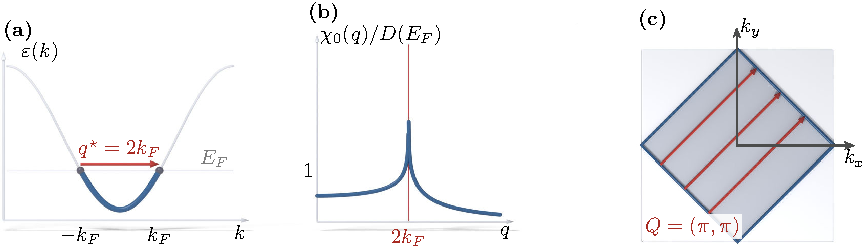
\includegraphics{figures/pdf/s09f01_nesting.pdf}
\end{aqmfigure}
